
\section{Results}

In this section the area, delay and power consumption for both a 50\%-pipelined and a non-pipelined version of the Wallace tree have been reported. The comparison has been performed for different numbers of bits and for different numbers of input operands and refers to a radix 2 multiplier implementation, where  the partial product terms to be added are placed as in Figure \ref{fig:wallace_tree}.
\begin{figure}[H]
	\centering
	\hspace{1 cm}
	\textsf{{\fontsize{9pt}{5.5pt}
			\begin{pgfpicture}{0cm}{0cm}{316pt}{393pt}
% Created by FidoCadJ ver. 0.24.6, export filter by Davide Bucci
\pgfsetxvec{\pgfpoint{1pt}{0pt}}
\pgfsetyvec{\pgfpoint{0pt}{1pt}}
\pgfsetroundjoin 
\pgfsetroundcap
\pgftranslateto{\pgfxy(0,393)}
\begin{pgfmagnify}{1}{-1}
% Layer color definitions
\definecolor{layer0}{rgb}{0.0,0.0,0.0}
\definecolor{layer1}{rgb}{0.0,0.0,0.5}
\definecolor{layer2}{rgb}{1.0,0.0,0.0}
\definecolor{layer3}{rgb}{0.0,0.5,0.5}
\definecolor{layer4}{rgb}{1.0,0.78,0.0}
\definecolor{layer5}{rgb}{0.5,1.0,0.0}
\definecolor{layer6}{rgb}{0.0,1.0,1.0}
\definecolor{layer7}{rgb}{0.0,0.5,0.0}
\definecolor{layer8}{rgb}{0.6,0.8,0.2}
\definecolor{layer9}{rgb}{1.0,0.08,0.58}
\definecolor{layer10}{rgb}{0.71,0.61,0.05}
\definecolor{layer11}{rgb}{0.0,0.5,1.0}
\definecolor{layer12}{rgb}{0.88,0.88,0.88}
\definecolor{layer13}{rgb}{0.64,0.64,0.64}
\definecolor{layer14}{rgb}{0.37,0.37,0.37}
\definecolor{layer15}{rgb}{0.0,0.0,0.0}
% End of color definitions
\color{layer0}
\pgfsetlinewidth{0.33pt}
\pgfcircle[fill]{\pgfxy(215,12)}{1.4pt}\pgfcircle[fill]{\pgfxy(201,12)}{1.4pt}\pgfcircle[fill]{\pgfxy(187,12)}{1.4pt}\pgfcircle[fill]{\pgfxy(173,12)}{1.4pt}\pgfcircle[fill]{\pgfxy(159,12)}{1.4pt}\pgfcircle[fill]{\pgfxy(145,12)}{1.4pt}\pgfcircle[fill]{\pgfxy(131,12)}{1.4pt}\pgfcircle[fill]{\pgfxy(117,12)}{1.4pt}\pgfcircle[fill]{\pgfxy(201,26)}{1.4pt}\pgfcircle[fill]{\pgfxy(187,26)}{1.4pt}\pgfcircle[fill]{\pgfxy(173,26)}{1.4pt}\pgfcircle[fill]{\pgfxy(159,26)}{1.4pt}\pgfcircle[fill]{\pgfxy(145,26)}{1.4pt}\pgfcircle[fill]{\pgfxy(131,26)}{1.4pt}\pgfcircle[fill]{\pgfxy(117,26)}{1.4pt}\pgfcircle[fill]{\pgfxy(103,26)}{1.4pt}\pgfcircle[fill]{\pgfxy(187,40)}{1.4pt}\pgfcircle[fill]{\pgfxy(173,40)}{1.4pt}\pgfcircle[fill]{\pgfxy(159,40)}{1.4pt}\pgfcircle[fill]{\pgfxy(145,40)}{1.4pt}\pgfcircle[fill]{\pgfxy(131,40)}{1.4pt}\pgfcircle[fill]{\pgfxy(117,40)}{1.4pt}\pgfcircle[fill]{\pgfxy(103,40)}{1.4pt}\pgfcircle[fill]{\pgfxy(89,40)}{1.4pt}\pgfcircle[fill]{\pgfxy(173,54)}{1.4pt}\pgfcircle[fill]{\pgfxy(159,54)}{1.4pt}\pgfcircle[fill]{\pgfxy(145,54)}{1.4pt}\pgfcircle[fill]{\pgfxy(131,54)}{1.4pt}\pgfcircle[fill]{\pgfxy(117,54)}{1.4pt}\pgfcircle[fill]{\pgfxy(103,54)}{1.4pt}\pgfcircle[fill]{\pgfxy(89,54)}{1.4pt}\pgfcircle[fill]{\pgfxy(75,54)}{1.4pt}\pgfcircle[fill]{\pgfxy(159,68)}{1.4pt}\pgfcircle[fill]{\pgfxy(145,68)}{1.4pt}\pgfcircle[fill]{\pgfxy(131,68)}{1.4pt}\pgfcircle[fill]{\pgfxy(117,68)}{1.4pt}\pgfcircle[fill]{\pgfxy(103,68)}{1.4pt}\pgfcircle[fill]{\pgfxy(89,68)}{1.4pt}\pgfcircle[fill]{\pgfxy(75,68)}{1.4pt}\pgfcircle[fill]{\pgfxy(61,68)}{1.4pt}\pgfcircle[fill]{\pgfxy(145,82)}{1.4pt}\pgfcircle[fill]{\pgfxy(131,82)}{1.4pt}\pgfcircle[fill]{\pgfxy(117,82)}{1.4pt}\pgfcircle[fill]{\pgfxy(103,82)}{1.4pt}\pgfcircle[fill]{\pgfxy(89,82)}{1.4pt}\pgfcircle[fill]{\pgfxy(75,82)}{1.4pt}\pgfcircle[fill]{\pgfxy(61,82)}{1.4pt}\pgfcircle[fill]{\pgfxy(47,82)}{1.4pt}\pgfcircle[fill]{\pgfxy(131,96)}{1.4pt}\pgfcircle[fill]{\pgfxy(117,96)}{1.4pt}\pgfcircle[fill]{\pgfxy(103,96)}{1.4pt}\pgfcircle[fill]{\pgfxy(89,96)}{1.4pt}\pgfcircle[fill]{\pgfxy(75,96)}{1.4pt}\pgfcircle[fill]{\pgfxy(61,96)}{1.4pt}\pgfcircle[fill]{\pgfxy(47,96)}{1.4pt}\pgfcircle[fill]{\pgfxy(33,96)}{1.4pt}\pgfcircle[fill]{\pgfxy(117,110)}{1.4pt}\pgfcircle[fill]{\pgfxy(103,110)}{1.4pt}\pgfcircle[fill]{\pgfxy(89,110)}{1.4pt}\pgfcircle[fill]{\pgfxy(75,110)}{1.4pt}\pgfcircle[fill]{\pgfxy(61,110)}{1.4pt}\pgfcircle[fill]{\pgfxy(47,110)}{1.4pt}\pgfcircle[fill]{\pgfxy(33,110)}{1.4pt}\pgfcircle[fill]{\pgfxy(19,110)}{1.4pt}\pgfsetlinewidth{0.7pt}
\pgfline{\pgfxy(5.0,124.0)}{\pgfxy(222.0,124.0)}
\pgfsetlinewidth{0.33pt}
\pgfcircle[fill]{\pgfxy(201,306)}{1.4pt}\pgfcircle[fill]{\pgfxy(187,306)}{1.4pt}\pgfcircle[fill]{\pgfxy(173,306)}{1.4pt}\pgfcircle[fill]{\pgfxy(159,306)}{1.4pt}\pgfcircle[fill]{\pgfxy(145,306)}{1.4pt}\pgfcircle[fill]{\pgfxy(131,306)}{1.4pt}\pgfcircle[fill]{\pgfxy(117,306)}{1.4pt}\pgfcircle[fill]{\pgfxy(103,306)}{1.4pt}\pgfcircle[fill]{\pgfxy(89,306)}{1.4pt}\pgfcircle[fill]{\pgfxy(75,306)}{1.4pt}\pgfcircle[fill]{\pgfxy(61,306)}{1.4pt}\pgfcircle[fill]{\pgfxy(47,306)}{1.4pt}\pgfcircle[fill]{\pgfxy(33,306)}{1.4pt}\pgfcircle[fill]{\pgfxy(19,306)}{1.4pt}\pgfcircle[fill]{\pgfxy(159,320)}{1.4pt}\pgfcircle[fill]{\pgfxy(145,320)}{1.4pt}\pgfcircle[fill]{\pgfxy(215,138)}{1.4pt}\pgfcircle[fill]{\pgfxy(201,138)}{1.4pt}\pgfcircle[fill]{\pgfxy(187,138)}{1.4pt}\pgfcircle[fill]{\pgfxy(173,138)}{1.4pt}\pgfcircle[fill]{\pgfxy(159,138)}{1.4pt}\pgfcircle[fill]{\pgfxy(145,138)}{1.4pt}\pgfcircle[fill]{\pgfxy(131,138)}{1.4pt}\pgfcircle[fill]{\pgfxy(117,138)}{1.4pt}\pgfcircle[fill]{\pgfxy(103,138)}{1.4pt}\pgfcircle[fill]{\pgfxy(89,138)}{1.4pt}\pgfcircle[fill]{\pgfxy(187,152)}{1.4pt}\pgfcircle[fill]{\pgfxy(173,152)}{1.4pt}\pgfcircle[fill]{\pgfxy(159,152)}{1.4pt}\pgfcircle[fill]{\pgfxy(145,152)}{1.4pt}\pgfcircle[fill]{\pgfxy(131,152)}{1.4pt}\pgfcircle[fill]{\pgfxy(117,152)}{1.4pt}\pgfcircle[fill]{\pgfxy(103,152)}{1.4pt}\pgfcircle[fill]{\pgfxy(89,152)}{1.4pt}\pgfcircle[fill]{\pgfxy(173,166)}{1.4pt}\pgfcircle[fill]{\pgfxy(159,166)}{1.4pt}\pgfcircle[fill]{\pgfxy(145,166)}{1.4pt}\pgfcircle[fill]{\pgfxy(131,166)}{1.4pt}\pgfcircle[fill]{\pgfxy(117,166)}{1.4pt}\pgfcircle[fill]{\pgfxy(103,166)}{1.4pt}\pgfcircle[fill]{\pgfxy(89,166)}{1.4pt}\pgfcircle[fill]{\pgfxy(75,166)}{1.4pt}\pgfcircle[fill]{\pgfxy(61,166)}{1.4pt}\pgfcircle[fill]{\pgfxy(47,166)}{1.4pt}\pgfcircle[fill]{\pgfxy(145,180)}{1.4pt}\pgfcircle[fill]{\pgfxy(131,180)}{1.4pt}\pgfcircle[fill]{\pgfxy(117,180)}{1.4pt}\pgfcircle[fill]{\pgfxy(103,180)}{1.4pt}\pgfcircle[fill]{\pgfxy(89,180)}{1.4pt}\pgfcircle[fill]{\pgfxy(75,180)}{1.4pt}\pgfcircle[fill]{\pgfxy(61,180)}{1.4pt}\pgfcircle[fill]{\pgfxy(47,180)}{1.4pt}\pgfcircle[fill]{\pgfxy(131,194)}{1.4pt}\pgfcircle[fill]{\pgfxy(117,194)}{1.4pt}\pgfcircle[fill]{\pgfxy(103,194)}{1.4pt}\pgfcircle[fill]{\pgfxy(89,194)}{1.4pt}\pgfcircle[fill]{\pgfxy(75,194)}{1.4pt}\pgfcircle[fill]{\pgfxy(61,194)}{1.4pt}\pgfcircle[fill]{\pgfxy(47,194)}{1.4pt}\pgfcircle[fill]{\pgfxy(33,194)}{1.4pt}\pgfcircle[fill]{\pgfxy(117,208)}{1.4pt}\pgfcircle[fill]{\pgfxy(103,208)}{1.4pt}\pgfcircle[fill]{\pgfxy(89,208)}{1.4pt}\pgfcircle[fill]{\pgfxy(75,208)}{1.4pt}\pgfcircle[fill]{\pgfxy(61,208)}{1.4pt}\pgfcircle[fill]{\pgfxy(47,208)}{1.4pt}\pgfcircle[fill]{\pgfxy(33,208)}{1.4pt}\pgfcircle[fill]{\pgfxy(19,208)}{1.4pt}\pgfsetlinewidth{0.7pt}
\pgfline{\pgfxy(5.0,222.0)}{\pgfxy(222.0,222.0)}
\pgfsetlinewidth{0.33pt}
\pgfcircle[fill]{\pgfxy(5,376)}{1.4pt}\pgfsetlinewidth{0.7pt}
\pgfline{\pgfxy(5.0,390.0)}{\pgfxy(222.0,390.0)}
\pgfsetlinewidth{0.33pt}
\pgfcircle[fill]{\pgfxy(75,250)}{1.4pt}\pgfcircle[fill]{\pgfxy(145,264)}{1.4pt}\pgfcircle[fill]{\pgfxy(131,264)}{1.4pt}\pgfcircle[fill]{\pgfxy(117,264)}{1.4pt}\pgfcircle[fill]{\pgfxy(103,264)}{1.4pt}\pgfcircle[fill]{\pgfxy(89,264)}{1.4pt}\pgfcircle[fill]{\pgfxy(75,264)}{1.4pt}\pgfcircle[fill]{\pgfxy(61,264)}{1.4pt}\pgfcircle[fill]{\pgfxy(47,264)}{1.4pt}\pgfcircle[fill]{\pgfxy(33,264)}{1.4pt}\pgfcircle[fill]{\pgfxy(19,264)}{1.4pt}\pgfcircle[fill]{\pgfxy(117,278)}{1.4pt}\pgfcircle[fill]{\pgfxy(103,278)}{1.4pt}\pgfcircle[fill]{\pgfxy(131,320)}{1.4pt}\pgfcircle[fill]{\pgfxy(215,236)}{1.4pt}\pgfcircle[fill]{\pgfxy(201,236)}{1.4pt}\pgfcircle[fill]{\pgfxy(187,236)}{1.4pt}\pgfcircle[fill]{\pgfxy(173,236)}{1.4pt}\pgfcircle[fill]{\pgfxy(159,236)}{1.4pt}\pgfcircle[fill]{\pgfxy(145,236)}{1.4pt}\pgfcircle[fill]{\pgfxy(131,236)}{1.4pt}\pgfcircle[fill]{\pgfxy(117,236)}{1.4pt}\pgfcircle[fill]{\pgfxy(103,236)}{1.4pt}\pgfcircle[fill]{\pgfxy(89,236)}{1.4pt}\pgfcircle[fill]{\pgfxy(75,236)}{1.4pt}\pgfcircle[fill]{\pgfxy(61,236)}{1.4pt}\pgfcircle[fill]{\pgfxy(47,236)}{1.4pt}\pgfcircle[fill]{\pgfxy(173,250)}{1.4pt}\pgfcircle[fill]{\pgfxy(159,250)}{1.4pt}\pgfcircle[fill]{\pgfxy(145,250)}{1.4pt}\pgfcircle[fill]{\pgfxy(131,250)}{1.4pt}\pgfcircle[fill]{\pgfxy(117,250)}{1.4pt}\pgfcircle[fill]{\pgfxy(103,250)}{1.4pt}\pgfcircle[fill]{\pgfxy(89,250)}{1.4pt}\pgfcircle[fill]{\pgfxy(33,278)}{1.4pt}\pgfcircle[fill]{\pgfxy(19,278)}{1.4pt}\pgfsetlinewidth{0.7pt}
\pgfline{\pgfxy(5.0,292.0)}{\pgfxy(222.0,292.0)}
\pgfsetlinewidth{0.33pt}
\pgfcircle[fill]{\pgfxy(33,362)}{1.4pt}\pgfcircle[fill]{\pgfxy(19,362)}{1.4pt}\pgfcircle[fill]{\pgfxy(145,376)}{1.4pt}\pgfcircle[fill]{\pgfxy(131,376)}{1.4pt}\pgfcircle[fill]{\pgfxy(215,362)}{1.4pt}\pgfcircle[fill]{\pgfxy(201,362)}{1.4pt}\pgfcircle[fill]{\pgfxy(187,362)}{1.4pt}\pgfcircle[fill]{\pgfxy(173,362)}{1.4pt}\pgfcircle[fill]{\pgfxy(159,362)}{1.4pt}\pgfcircle[fill]{\pgfxy(145,362)}{1.4pt}\pgfcircle[fill]{\pgfxy(89,278)}{1.4pt}\pgfcircle[fill]{\pgfxy(75,278)}{1.4pt}\pgfcircle[fill]{\pgfxy(61,278)}{1.4pt}\pgfcircle[fill]{\pgfxy(47,278)}{1.4pt}\pgfcircle[fill]{\pgfxy(75,320)}{1.4pt}\pgfcircle[fill]{\pgfxy(61,320)}{1.4pt}\pgfcircle[fill]{\pgfxy(47,320)}{1.4pt}\pgfcircle[fill]{\pgfxy(33,320)}{1.4pt}\pgfcircle[fill]{\pgfxy(117,334)}{1.4pt}\pgfcircle[fill]{\pgfxy(103,334)}{1.4pt}\pgfcircle[fill]{\pgfxy(89,334)}{1.4pt}\pgfcircle[fill]{\pgfxy(117,376)}{1.4pt}\pgfcircle[fill]{\pgfxy(103,376)}{1.4pt}\pgfcircle[fill]{\pgfxy(89,376)}{1.4pt}\pgfcircle[fill]{\pgfxy(75,376)}{1.4pt}\pgfcircle[fill]{\pgfxy(61,376)}{1.4pt}\pgfcircle[fill]{\pgfxy(47,376)}{1.4pt}\pgfcircle[fill]{\pgfxy(215,306)}{1.4pt}\pgfcircle[fill]{\pgfxy(19,376)}{1.4pt}\pgfcircle[fill]{\pgfxy(103,320)}{1.4pt}\pgfcircle[fill]{\pgfxy(89,320)}{1.4pt}\pgfcircle[fill]{\pgfxy(75,362)}{1.4pt}\pgfcircle[fill]{\pgfxy(61,362)}{1.4pt}\pgfcircle[fill]{\pgfxy(47,362)}{1.4pt}\pgfcircle[fill]{\pgfxy(19,334)}{1.4pt}\pgfsetlinewidth{0.7pt}
\pgfline{\pgfxy(5.0,348.0)}{\pgfxy(222.0,348.0)}
\pgfsetlinewidth{0.33pt}
\pgfcircle[fill]{\pgfxy(131,362)}{1.4pt}\pgfcircle[fill]{\pgfxy(117,320)}{1.4pt}\pgfcircle[fill]{\pgfxy(75,334)}{1.4pt}\pgfcircle[fill]{\pgfxy(61,334)}{1.4pt}\pgfcircle[fill]{\pgfxy(47,334)}{1.4pt}\pgfcircle[fill]{\pgfxy(33,334)}{1.4pt}\pgfcircle[fill]{\pgfxy(103,362)}{1.4pt}\pgfcircle[fill]{\pgfxy(89,362)}{1.4pt}\pgfcircle[fill]{\pgfxy(117,362)}{1.4pt}\pgfcircle[fill]{\pgfxy(33,376)}{1.4pt}\begin{pgfmagnify}{1}{-1}
\pgfputat{\pgfxy(265,-159)}{\pgfbox[left,top]{Half Adder}}
\end{pgfmagnify}
\begin{pgfmagnify}{1}{-1}
\pgfputat{\pgfxy(265,-229)}{\pgfbox[left,top]{Full Adder}}
\end{pgfmagnify}
\color{layer1}
\pgfsetlinewidth{0.7pt}
\pgfmoveto{\pgfxy(141,131)}
\pgflineto{\pgfxy(149,131)}
\pgflineto{\pgfxy(149,173)}
\pgflineto{\pgfxy(141,173)}
\pgfclosepath 
\pgfqstroke 
\pgfmoveto{\pgfxy(85,131)}
\pgflineto{\pgfxy(93,131)}
\pgflineto{\pgfxy(93,173)}
\pgflineto{\pgfxy(85,173)}
\pgfclosepath 
\pgfqstroke 
\pgfmoveto{\pgfxy(99,131)}
\pgflineto{\pgfxy(107,131)}
\pgflineto{\pgfxy(107,173)}
\pgflineto{\pgfxy(99,173)}
\pgfclosepath 
\pgfqstroke 
\pgfmoveto{\pgfxy(155,131)}
\pgflineto{\pgfxy(163,131)}
\pgflineto{\pgfxy(163,173)}
\pgflineto{\pgfxy(155,173)}
\pgfclosepath 
\pgfqstroke 
\pgfsetdash{{1.0pt}{1.0pt}}{0pt}
\pgfmoveto{\pgfxy(127,173)}
\pgflineto{\pgfxy(135,173)}
\pgflineto{\pgfxy(135,215)}
\pgflineto{\pgfxy(127,215)}
\pgfclosepath 
\pgfqstroke 
\pgfsetdash{}{0pt}
\pgfmoveto{\pgfxy(127,131)}
\pgflineto{\pgfxy(135,131)}
\pgflineto{\pgfxy(135,173)}
\pgflineto{\pgfxy(127,173)}
\pgfclosepath 
\pgfqstroke 
\pgfmoveto{\pgfxy(113,173)}
\pgflineto{\pgfxy(121,173)}
\pgflineto{\pgfxy(121,215)}
\pgflineto{\pgfxy(113,215)}
\pgfclosepath 
\pgfqstroke 
\pgfmoveto{\pgfxy(99,173)}
\pgflineto{\pgfxy(107,173)}
\pgflineto{\pgfxy(107,215)}
\pgflineto{\pgfxy(99,215)}
\pgfclosepath 
\pgfqstroke 
\pgfmoveto{\pgfxy(85,173)}
\pgflineto{\pgfxy(93,173)}
\pgflineto{\pgfxy(93,215)}
\pgflineto{\pgfxy(85,215)}
\pgfclosepath 
\pgfqstroke 
\pgfmoveto{\pgfxy(71,173)}
\pgflineto{\pgfxy(79,173)}
\pgflineto{\pgfxy(79,215)}
\pgflineto{\pgfxy(71,215)}
\pgfclosepath 
\pgfqstroke 
\pgfmoveto{\pgfxy(57,173)}
\pgflineto{\pgfxy(65,173)}
\pgflineto{\pgfxy(65,215)}
\pgflineto{\pgfxy(57,215)}
\pgfclosepath 
\pgfqstroke 
\pgfmoveto{\pgfxy(43,173)}
\pgflineto{\pgfxy(51,173)}
\pgflineto{\pgfxy(51,215)}
\pgflineto{\pgfxy(43,215)}
\pgfclosepath 
\pgfqstroke 
\pgfsetdash{{1.0pt}{1.0pt}}{0pt}
\pgfmoveto{\pgfxy(155,47)}
\pgflineto{\pgfxy(163,47)}
\pgflineto{\pgfxy(163,89)}
\pgflineto{\pgfxy(155,89)}
\pgfclosepath 
\pgfqstroke 
\pgfsetdash{}{0pt}
\pgfmoveto{\pgfxy(141,47)}
\pgflineto{\pgfxy(149,47)}
\pgflineto{\pgfxy(149,89)}
\pgflineto{\pgfxy(141,89)}
\pgfclosepath 
\pgfqstroke 
\pgfmoveto{\pgfxy(183,5)}
\pgflineto{\pgfxy(191,5)}
\pgflineto{\pgfxy(191,47)}
\pgflineto{\pgfxy(183,47)}
\pgfclosepath 
\pgfqstroke 
\pgfmoveto{\pgfxy(169,5)}
\pgflineto{\pgfxy(177,5)}
\pgflineto{\pgfxy(177,47)}
\pgflineto{\pgfxy(169,47)}
\pgfclosepath 
\pgfqstroke 
\pgfmoveto{\pgfxy(155,5)}
\pgflineto{\pgfxy(163,5)}
\pgflineto{\pgfxy(163,47)}
\pgflineto{\pgfxy(155,47)}
\pgfclosepath 
\pgfqstroke 
\pgfmoveto{\pgfxy(141,5)}
\pgflineto{\pgfxy(149,5)}
\pgflineto{\pgfxy(149,47)}
\pgflineto{\pgfxy(141,47)}
\pgfclosepath 
\pgfqstroke 
\pgfmoveto{\pgfxy(113,131)}
\pgflineto{\pgfxy(121,131)}
\pgflineto{\pgfxy(121,173)}
\pgflineto{\pgfxy(113,173)}
\pgfclosepath 
\pgfqstroke 
\pgfmoveto{\pgfxy(113,5)}
\pgflineto{\pgfxy(121,5)}
\pgflineto{\pgfxy(121,47)}
\pgflineto{\pgfxy(113,47)}
\pgfclosepath 
\pgfqstroke 
\pgfsetdash{{1.0pt}{1.0pt}}{0pt}
\pgfmoveto{\pgfxy(99,5)}
\pgflineto{\pgfxy(107,5)}
\pgflineto{\pgfxy(107,47)}
\pgflineto{\pgfxy(99,47)}
\pgfclosepath 
\pgfqstroke 
\pgfsetdash{}{0pt}
\pgfmoveto{\pgfxy(29,299)}
\pgflineto{\pgfxy(37,299)}
\pgflineto{\pgfxy(37,341)}
\pgflineto{\pgfxy(29,341)}
\pgfclosepath 
\pgfqstroke 
\pgfsetdash{{1.0pt}{1.0pt}}{0pt}
\pgfmoveto{\pgfxy(15,299)}
\pgflineto{\pgfxy(23,299)}
\pgflineto{\pgfxy(23,341)}
\pgflineto{\pgfxy(15,341)}
\pgfclosepath 
\pgfqstroke 
\pgfsetdash{}{0pt}
\pgfmoveto{\pgfxy(127,47)}
\pgflineto{\pgfxy(135,47)}
\pgflineto{\pgfxy(135,89)}
\pgflineto{\pgfxy(127,89)}
\pgfclosepath 
\pgfqstroke 
\pgfmoveto{\pgfxy(113,47)}
\pgflineto{\pgfxy(121,47)}
\pgflineto{\pgfxy(121,89)}
\pgflineto{\pgfxy(113,89)}
\pgfclosepath 
\pgfqstroke 
\pgfmoveto{\pgfxy(99,47)}
\pgflineto{\pgfxy(107,47)}
\pgflineto{\pgfxy(107,89)}
\pgflineto{\pgfxy(99,89)}
\pgfclosepath 
\pgfqstroke 
\pgfmoveto{\pgfxy(85,47)}
\pgflineto{\pgfxy(93,47)}
\pgflineto{\pgfxy(93,89)}
\pgflineto{\pgfxy(85,89)}
\pgfclosepath 
\pgfqstroke 
\pgfmoveto{\pgfxy(71,47)}
\pgflineto{\pgfxy(79,47)}
\pgflineto{\pgfxy(79,89)}
\pgflineto{\pgfxy(71,89)}
\pgfclosepath 
\pgfqstroke 
\pgfsetdash{{1.0pt}{1.0pt}}{0pt}
\pgfmoveto{\pgfxy(57,47)}
\pgflineto{\pgfxy(65,47)}
\pgflineto{\pgfxy(65,89)}
\pgflineto{\pgfxy(57,89)}
\pgfclosepath 
\pgfqstroke 
\pgfmoveto{\pgfxy(29,173)}
\pgflineto{\pgfxy(37,173)}
\pgflineto{\pgfxy(37,215)}
\pgflineto{\pgfxy(29,215)}
\pgfclosepath 
\pgfqstroke 
\pgfmoveto{\pgfxy(141,299)}
\pgflineto{\pgfxy(149,299)}
\pgflineto{\pgfxy(149,341)}
\pgflineto{\pgfxy(141,341)}
\pgfclosepath 
\pgfqstroke 
\pgfmoveto{\pgfxy(127,299)}
\pgflineto{\pgfxy(135,299)}
\pgflineto{\pgfxy(135,341)}
\pgflineto{\pgfxy(127,341)}
\pgfclosepath 
\pgfqstroke 
\pgfsetdash{}{0pt}
\pgfmoveto{\pgfxy(113,299)}
\pgflineto{\pgfxy(121,299)}
\pgflineto{\pgfxy(121,341)}
\pgflineto{\pgfxy(113,341)}
\pgfclosepath 
\pgfqstroke 
\pgfmoveto{\pgfxy(99,299)}
\pgflineto{\pgfxy(107,299)}
\pgflineto{\pgfxy(107,341)}
\pgflineto{\pgfxy(99,341)}
\pgfclosepath 
\pgfqstroke 
\pgfmoveto{\pgfxy(85,299)}
\pgflineto{\pgfxy(93,299)}
\pgflineto{\pgfxy(93,341)}
\pgflineto{\pgfxy(85,341)}
\pgfclosepath 
\pgfqstroke 
\pgfmoveto{\pgfxy(71,299)}
\pgflineto{\pgfxy(79,299)}
\pgflineto{\pgfxy(79,341)}
\pgflineto{\pgfxy(71,341)}
\pgfclosepath 
\pgfqstroke 
\pgfsetdash{{1.0pt}{1.0pt}}{0pt}
\pgfmoveto{\pgfxy(169,229)}
\pgflineto{\pgfxy(177,229)}
\pgflineto{\pgfxy(177,271)}
\pgflineto{\pgfxy(169,271)}
\pgfclosepath 
\pgfqstroke 
\pgfmoveto{\pgfxy(155,229)}
\pgflineto{\pgfxy(163,229)}
\pgflineto{\pgfxy(163,271)}
\pgflineto{\pgfxy(155,271)}
\pgfclosepath 
\pgfqstroke 
\pgfsetdash{}{0pt}
\pgfmoveto{\pgfxy(141,229)}
\pgflineto{\pgfxy(149,229)}
\pgflineto{\pgfxy(149,271)}
\pgflineto{\pgfxy(141,271)}
\pgfclosepath 
\pgfqstroke 
\pgfmoveto{\pgfxy(127,229)}
\pgflineto{\pgfxy(135,229)}
\pgflineto{\pgfxy(135,271)}
\pgflineto{\pgfxy(127,271)}
\pgfclosepath 
\pgfqstroke 
\pgfmoveto{\pgfxy(113,229)}
\pgflineto{\pgfxy(121,229)}
\pgflineto{\pgfxy(121,271)}
\pgflineto{\pgfxy(113,271)}
\pgfclosepath 
\pgfqstroke 
\pgfmoveto{\pgfxy(99,229)}
\pgflineto{\pgfxy(107,229)}
\pgflineto{\pgfxy(107,271)}
\pgflineto{\pgfxy(99,271)}
\pgfclosepath 
\pgfqstroke 
\pgfmoveto{\pgfxy(85,229)}
\pgflineto{\pgfxy(93,229)}
\pgflineto{\pgfxy(93,271)}
\pgflineto{\pgfxy(85,271)}
\pgfclosepath 
\pgfqstroke 
\pgfmoveto{\pgfxy(71,229)}
\pgflineto{\pgfxy(79,229)}
\pgflineto{\pgfxy(79,271)}
\pgflineto{\pgfxy(71,271)}
\pgfclosepath 
\pgfqstroke 
\pgfsetdash{{1.0pt}{1.0pt}}{0pt}
\pgfmoveto{\pgfxy(57,229)}
\pgflineto{\pgfxy(65,229)}
\pgflineto{\pgfxy(65,271)}
\pgflineto{\pgfxy(57,271)}
\pgfclosepath 
\pgfqstroke 
\pgfmoveto{\pgfxy(43,229)}
\pgflineto{\pgfxy(51,229)}
\pgflineto{\pgfxy(51,271)}
\pgflineto{\pgfxy(43,271)}
\pgfclosepath 
\pgfqstroke 
\pgfmoveto{\pgfxy(155,299)}
\pgflineto{\pgfxy(163,299)}
\pgflineto{\pgfxy(163,341)}
\pgflineto{\pgfxy(155,341)}
\pgfclosepath 
\pgfqstroke 
\pgfmoveto{\pgfxy(197,5)}
\pgflineto{\pgfxy(205,5)}
\pgflineto{\pgfxy(205,47)}
\pgflineto{\pgfxy(197,47)}
\pgfclosepath 
\pgfqstroke 
\pgfmoveto{\pgfxy(183,131)}
\pgflineto{\pgfxy(191,131)}
\pgflineto{\pgfxy(191,173)}
\pgflineto{\pgfxy(183,173)}
\pgfclosepath 
\pgfqstroke 
\pgfsetdash{}{0pt}
\pgfmoveto{\pgfxy(169,131)}
\pgflineto{\pgfxy(177,131)}
\pgflineto{\pgfxy(177,173)}
\pgflineto{\pgfxy(169,173)}
\pgfclosepath 
\pgfqstroke 
\pgfmoveto{\pgfxy(247,212)}
\pgflineto{\pgfxy(256,212)}
\pgflineto{\pgfxy(256,254)}
\pgflineto{\pgfxy(247,254)}
\pgfclosepath 
\pgfqstroke 
\pgfsetdash{{1.0pt}{1.0pt}}{0pt}
\pgfmoveto{\pgfxy(247,142)}
\pgflineto{\pgfxy(256,142)}
\pgflineto{\pgfxy(256,184)}
\pgflineto{\pgfxy(247,184)}
\pgfclosepath 
\pgfqstroke 
\pgfsetdash{}{0pt}
\pgfmoveto{\pgfxy(127,5)}
\pgflineto{\pgfxy(135,5)}
\pgflineto{\pgfxy(135,47)}
\pgflineto{\pgfxy(127,47)}
\pgfclosepath 
\pgfqstroke 
\pgfmoveto{\pgfxy(57,299)}
\pgflineto{\pgfxy(65,299)}
\pgflineto{\pgfxy(65,341)}
\pgflineto{\pgfxy(57,341)}
\pgfclosepath 
\pgfqstroke 
\pgfmoveto{\pgfxy(43,299)}
\pgflineto{\pgfxy(51,299)}
\pgflineto{\pgfxy(51,341)}
\pgflineto{\pgfxy(43,341)}
\pgfclosepath 
\pgfqstroke 
\end{pgfmagnify}
\end{pgfpicture}}}
	\caption{Wallace Tree with $ n=8 $, $ k=8 $}
	\label{fig:wallace_tree}
\end{figure}


\subsection{Area}

	\begin{figure}[H]
		\makebox[\textwidth][c]{
			\begin{subfigure}{0.55\textwidth}
					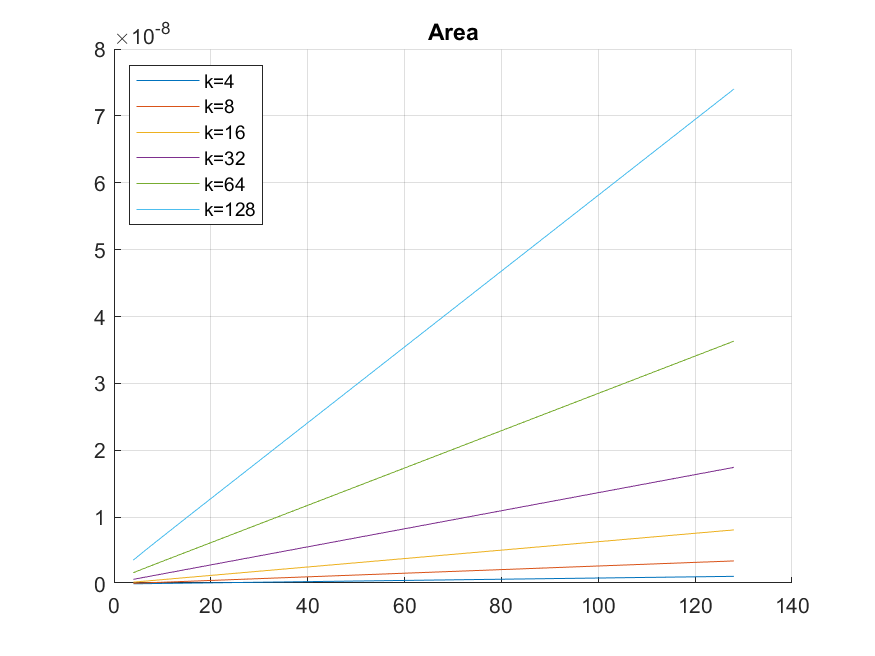
\includegraphics[width=9cm]{immagini/radix2ppipe0/area.png}
					\caption{Non-pipelined version}
				%				\label{fig:area}
			\end{subfigure}
			\begin{subfigure}{0.55\textwidth}
				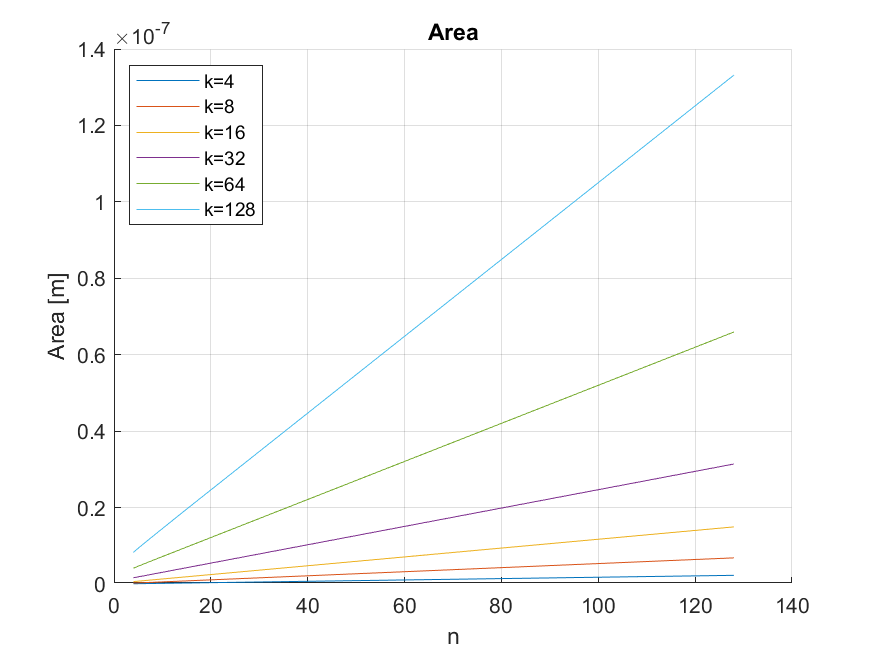
\includegraphics[width=9cm]{immagini/radix2ppipe2/area.png}
				\caption{50\%-Pipelined version}
%				\label{fig:3D area}
			\end{subfigure}
		
}{
		\begin{subfigure}{0.55\textwidth}
			\includegraphics[width=8cm]{immagini/radix2ppipe0/area3D.png}
			\caption{Non-pipelined version}
			%				\label{fig:area}
		\end{subfigure}
		\begin{subfigure}{0.55\textwidth}
			\includegraphics[width=8cm]{immagini/radix2ppipe2/area3D.png}
			\caption{50\%-Pipelined version}
			%				\label{fig:3D area}
		\end{subfigure}
	}
	\caption{Area}
	\label{fig:Area}
\end{figure}
As expected, the total area of the tree linearly increases with the number of bits (n) per input operand (Figures \ref{fig:Area}). The higher the number of operands (k) is, the larger is the total amount of the occupied area because of the higher number of stages required for the calculation.

In particular in order to appreciate the differences between the two versions of the tree, some meaningful points have been reported in the following table.


\begin{center}
\begin{tabular}{cc|c|c|}
	\cline{3-4}
	\multicolumn{1}{l}{}               & \multicolumn{1}{l|}{} & \multicolumn{2}{c|}{\textbf{Occupied area {[}m\textasciicircum{}2{]}}} \\ \hline
	\multicolumn{1}{|c|}{\textbf{n}}   & \textbf{k}            & \textbf{Non-pipelined}            & \textbf{50\% pipelined}            \\ \hline
	\multicolumn{1}{|c|}{\textbf{4}}   & \textbf{4}            & 3.4e-11                           & 6.504e-11                          \\ \hline
	\multicolumn{1}{|c|}{\textbf{4}}   & \textbf{128}          & 2.499e-9                          & 8.278e-9                           \\ \hline
	\multicolumn{1}{|c|}{\textbf{128}} & \textbf{4}            & 1.15e-9                           & 2.267e-9                           \\ \hline
	\multicolumn{1}{|c|}{\textbf{128}} & \textbf{128}          & 7.28e-8                           & 1.332e-7                           \\ \hline
\end{tabular}

\end{center}
As expected, the occupied area increases in the pipelind case since different levels of Flip flops are inserted; this increase becomes more and more significant as the number of bits and operands increase.



\subsection{Delay}

The delay is the time interval necessary to complete the computation through the whole tree.
In the non-pipelined case the path is entirely combinatorial while in the pipelined version the critical path is splitted into shorter homogeneous paths. In this last case the delay is therefore computed as the product between the clock period (the critical path delay) and the number of the pipeline stages inserted.

\begin{figure}[H]
	\makebox[\textwidth][c]{
		\begin{subfigure}{0.55\textwidth}
			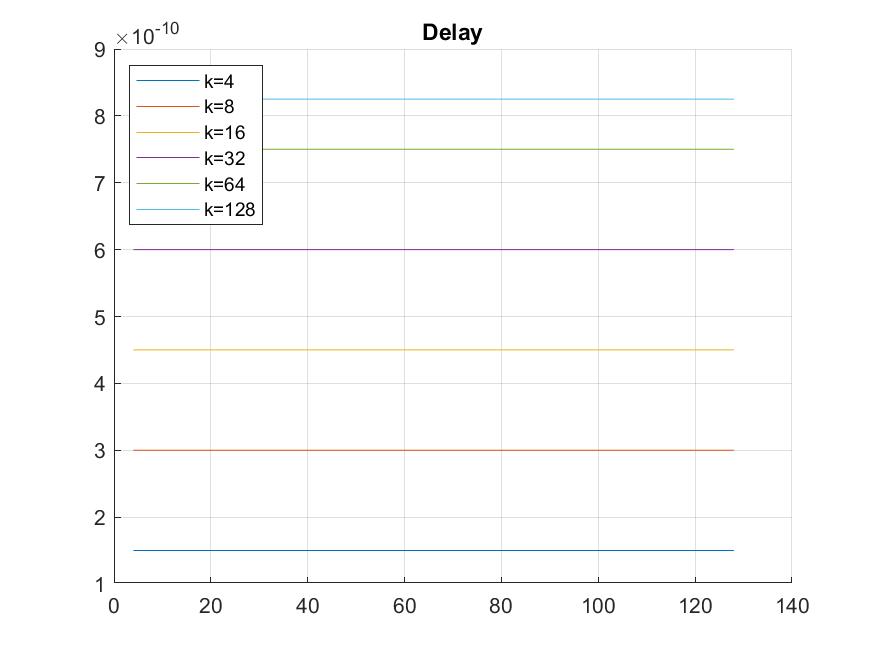
\includegraphics[width=9cm]{immagini/radix2ppipe0/delay.png}
			\caption{Non-pipelined version}
			%				\label{fig:area}
		\end{subfigure}
		\begin{subfigure}{0.55\textwidth}
			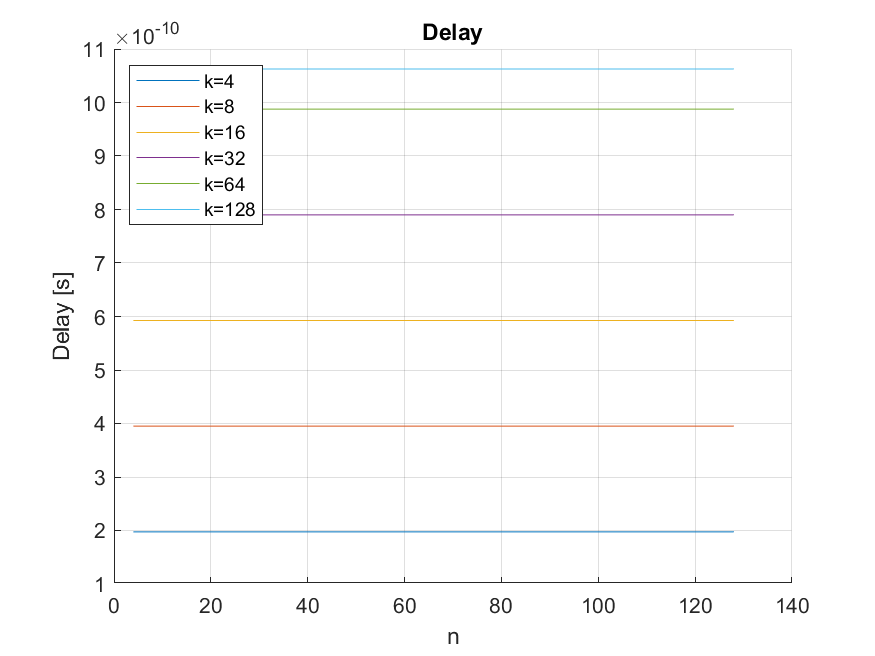
\includegraphics[width=9cm]{immagini/radix2ppipe2/delay.png}
			\caption{50\%-Pipelined version}
			%				\label{fig:3D area}
		\end{subfigure}
	}
{
		\begin{subfigure}{0.55\textwidth}
			\includegraphics[width=8cm]{immagini/radix2ppipe0/delay3D.png}
			\caption{Non-pipelined version}
			%				\label{fig:area}
		\end{subfigure}
		\begin{subfigure}{0.55\textwidth}
			\includegraphics[width=8cm]{immagini/radix2ppipe2/delay3D.png}
			\caption{50\%-Pipelined version}
			%				\label{fig:3D area}
		\end{subfigure}
	}
	\caption{Delay}
	\label{fig:Delay}
\end{figure}

As shown in Figure \ref{fig:Delay}, the amount of delay increases with the number of input operands, instead it is constant with respect to the number of bits. Since in each stage of the tree, full adders and half adders work in parallel, an higher input parallelism does not affect the total delay.

Once again, in order to appreciate the differences between the two versions of the tree, the delay has been computed for a growing number of operands.

\begin{center}
	\begin{tabular}{c|c|c|}
		\cline{2-3}
		\textbf{}                          & \multicolumn{2}{c|}{\textbf{Delay {[}ns{]}}}     \\ \hline
		\multicolumn{1}{|c|}{\textbf{k}}   & \textbf{Non-pipelined} & \textbf{50\% pipelined} \\ \hline
		\multicolumn{1}{|c|}{\textbf{4}}   & 0.15                   & 0.198                   \\ \hline
		\multicolumn{1}{|c|}{\textbf{8}}   & 0.3                    & 0.395                   \\ \hline
		\multicolumn{1}{|c|}{\textbf{16}}  & 0.45                   & 0.593                   \\ \hline
		\multicolumn{1}{|c|}{\textbf{32}}  & 0.6                    & 0.79                    \\ \hline
		\multicolumn{1}{|c|}{\textbf{64}}  & 0.75                   & 0.988                   \\ \hline
		\multicolumn{1}{|c|}{\textbf{128}} & 0.825                  & 1.063                    \\ \hline
	\end{tabular}
\end{center}

As expected, it is possible to notice how the delay increases in the pipelined case because of the overhead introduced by the registers stages. In particular, as k increases, also the number of levels of the tree increases and so more stages of flip flops are introduced.

\subsection{Static power}

Static power increases with both the number of bits and  the number of operands. This is trivial to understand why both of them depend on the total equivalent capacitance of the tree.
\begin{figure}[H]
	\makebox[\textwidth][c]{
		\begin{subfigure}{0.55\textwidth}
			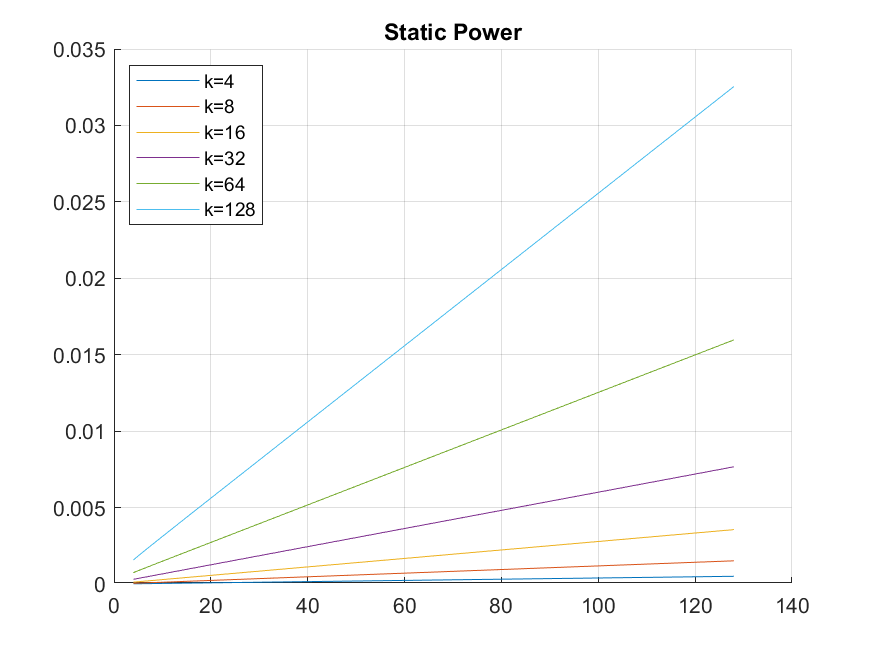
\includegraphics[width=9cm]{immagini/radix2ppipe0/p_static.png}
			\caption{Non-pipelined version}
			%				\label{fig:area}
		\end{subfigure}
		\begin{subfigure}{0.55\textwidth}
			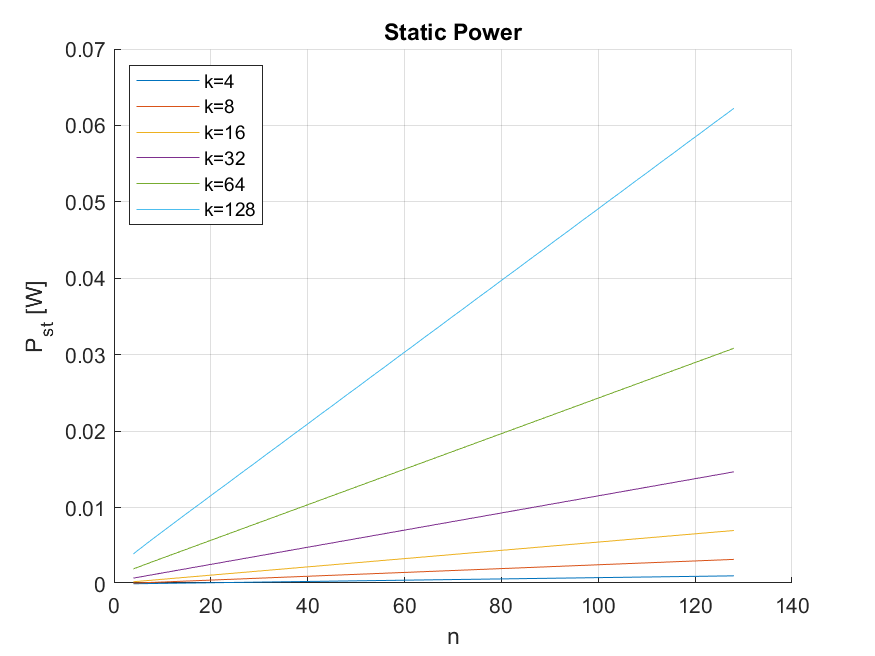
\includegraphics[width=9cm]{immagini/radix2ppipe2/p_static.png}
			\caption{50\%-Pipelined version}
			%				\label{fig:3D area}
		\end{subfigure}
	}
	{
		\begin{subfigure}{0.55\textwidth}
			\includegraphics[width=8cm]{immagini/radix2ppipe0/p_static3D.png}
			\caption{Non-pipelined version}
			%				\label{fig:area}
		\end{subfigure}
		\begin{subfigure}{0.55\textwidth}
			\includegraphics[width=8cm]{immagini/radix2ppipe2/p_static3D.png}
			\caption{50\%-Pipelined version}
			%				\label{fig:3D area}
		\end{subfigure}
	}
	\caption{Static power}
	\label{fig:pstat}
\end{figure}

Some quantitative evaluations are reported in the table below.

\begin{center}
	\begin{tabular}{cc|c|c|}
		\cline{3-4}
		\multicolumn{1}{l}{}               & \multicolumn{1}{l|}{} & \multicolumn{2}{c|}{\textbf{Static power {[}W{]}}} \\ \hline
		\multicolumn{1}{|c|}{\textbf{n}}   & \textbf{k}            & \textbf{Non-pipelined}  & \textbf{50\% pipelined} \\ \hline
		\multicolumn{1}{|c|}{\textbf{4}}   & \textbf{4}            & 1.495e-5                & 3.078e-5                \\ \hline
		\multicolumn{1}{|c|}{\textbf{4}}   & \textbf{128}          & 1.1e-3                  & 3.933e-3                \\ \hline
		\multicolumn{1}{|c|}{\textbf{128}} & \textbf{4}            & 5.057e-4                & 1.067e-3                \\ \hline
		\multicolumn{1}{|c|}{\textbf{128}} & \textbf{128}          & 3.2e-2                  & 6.224e-2                \\ \hline
	\end{tabular}
\end{center}

The pipelined version, again, is characterized by a larger static power consumption with respect to the non pipelined version since also the power consumption of the flip flops has been taken into account. 


\subsection{Dynamic power}
In order to make a proper comparison, dynamic power estimation has been performed for both versions of the tree considering an operating frequency of 5GHz.
\begin{figure}[H]
	\makebox[\textwidth][c]{
		\begin{subfigure}{0.55\textwidth}
			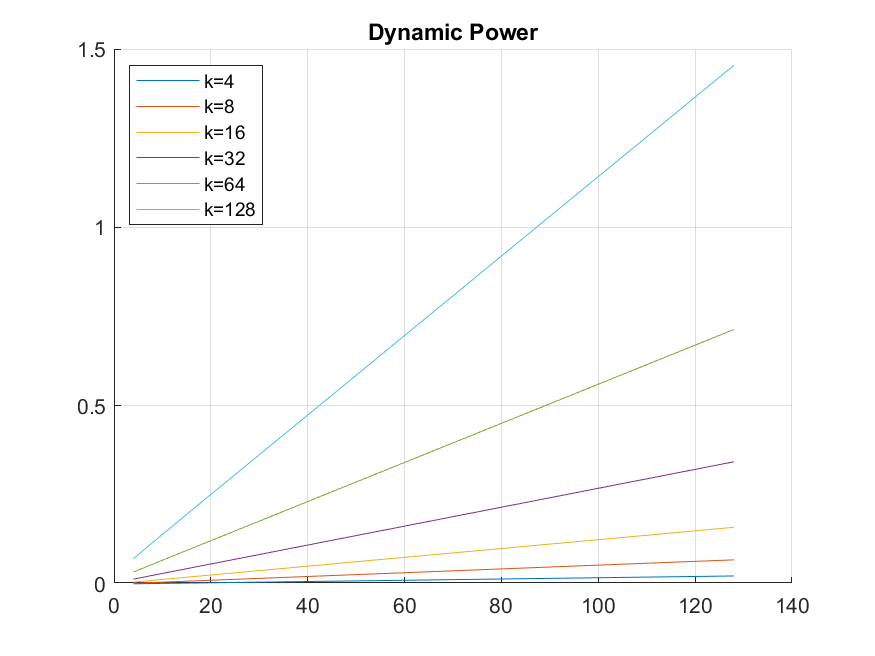
\includegraphics[width=9cm]{immagini/radix2ppipe0/p_dyn.png}
			\caption{Non-pipelined version}
			%				\label{fig:area}
		\end{subfigure}
		\begin{subfigure}{0.55\textwidth}
			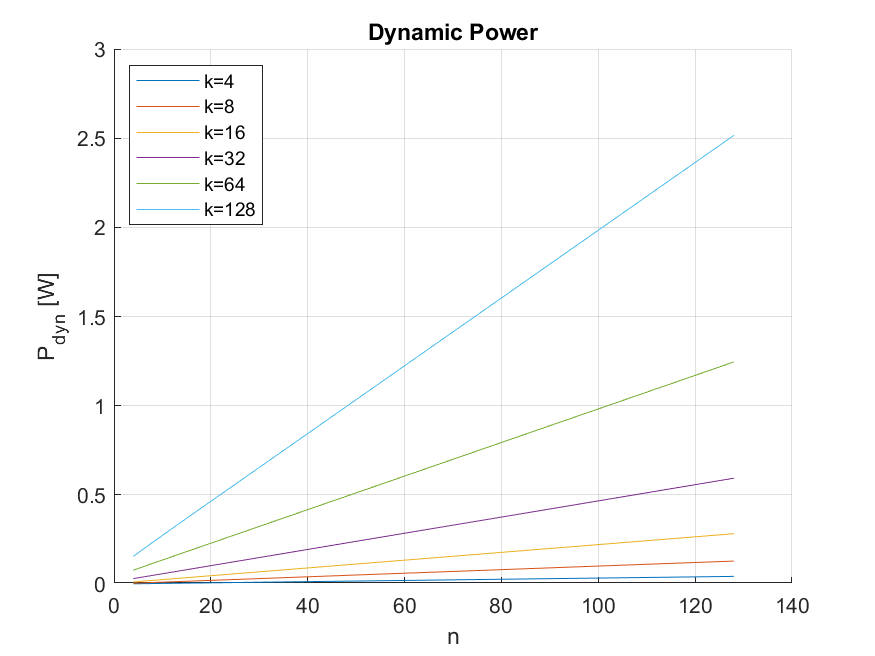
\includegraphics[width=9cm]{immagini/radix2ppipe2/p_dyn.png}
			\caption{50\%-Pipelined version}
			%				\label{fig:3D area}
		\end{subfigure}
	}
	{
		\begin{subfigure}{0.55\textwidth}
			\includegraphics[width=8cm]{immagini/radix2ppipe0/p_dyn3D.png}
			\caption{Non-pipelined version}
			%				\label{fig:area}
		\end{subfigure}
		\begin{subfigure}{0.55\textwidth}
			\includegraphics[width=8cm]{immagini/radix2ppipe2/p_dyn3D.png}
			\caption{50\%-Pipelined version}
			%				\label{fig:3D area}
		\end{subfigure}
	}
	\caption{Dynamic power ($f_{ck}=5 GHz$)}
	\label{fig:pdyn}
\end{figure}

In order to appreciate the differences between the two versions of the tree, some meaningful points have been reported in the following table.
\begin{center}
	\begin{tabular}{cc|c|c|}
		\cline{3-4}
		\multicolumn{1}{l}{}               & \multicolumn{1}{l|}{} & \multicolumn{2}{c|}{\textbf{Dynamic power {[}W{]}}} \\ \hline
		\multicolumn{1}{|c|}{\textbf{n}}   & \textbf{k}            & \textbf{Non-pipelined}   & \textbf{50\% pipelined}  \\ \hline
		\multicolumn{1}{|c|}{\textbf{4}}   & \textbf{4}            & 6.681e-4                 & 1.218e-3                 \\ \hline
		\multicolumn{1}{|c|}{\textbf{4}}   & \textbf{128}          & 0.049                    & 0.155                    \\ \hline
		\multicolumn{1}{|c|}{\textbf{128}} & \textbf{4}            & 0.023                    & 0.043                    \\ \hline
		\multicolumn{1}{|c|}{\textbf{128}} & \textbf{128}          & 1.431                    & 2.516                    \\ \hline
	\end{tabular}
\end{center}

Also in this case the power consumption grows with the number of bits-per-operand (n) and with the number of operands (k). 
In particular if n increases, the number of flip flops per level also increases; if k increases, the number of the stages of the tree and therefore the number of pipeline stages to be inserted increase. For this reason the pipelined version consumes more than the non-pipelined one.

Besides performing power estimations considering an operating frequency selected by the user, the developed script also is able to compute the maximum operating frequency depending on the critical path. It is possible to use then this value to obtain the dissipated power amount in the case of working at maximum performance.
In particular, considering the technological parameters involved, the system is able to work up to a $f_{ckMax}$ of about 5.06 GHz.

\subsection{Different pipeline percentages comparison}
The developed Matlab code also uses a parameter called $ppipe$: it is linked to the percentage of pipelining to be applied at the tree, in particular it indicates every how many levels of the tree a pipe stage is introduced. For example:
\begin{itemize}
	\item if $ppipe=0$ no pipeline stages are introduced (non-pipelined version);
	\item if $ppipe=1$ a pipeline stage is inserted at every level of the tree (fully pipelined version, 100\%);
	\item if $ppipe=2$ a pipeline stage is inserted every 2 levels of the tree (50\%).
\end{itemize}
In Figure \ref{fig:ppipe} occupied area, delay, static and dynamic power estimations are shown in the case of n=128, k=128 and a varying value of ppipe.
It is possible to observe that the plots are similar. When ppipe=0 no flip flops are inserted in the design, this corresponds to the minimum area and power.
When ppipe=1 the design is fully pipelined and therefore here lies the maximum for both area and power.
As the pipeline percentage decreases (ppipe increases) the plots approximately follow the trend of a decreasing exponential.

\begin{figure}[H]
	\makebox[\textwidth][c]{
		\begin{subfigure}{0.55\textwidth}
			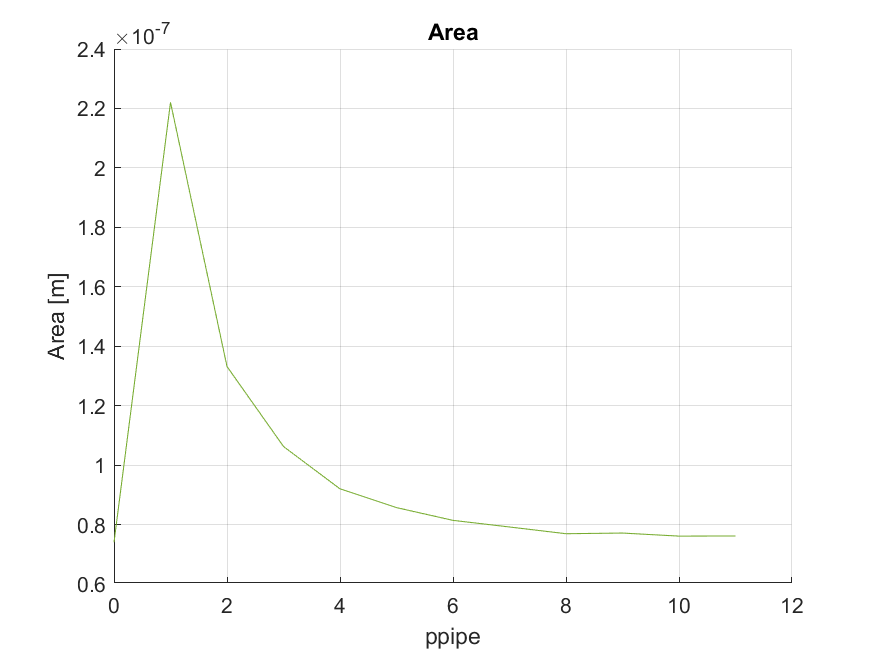
\includegraphics[width=9cm]{immagini/radix2ppipe2/area_pipe.png}
		\end{subfigure}
		\begin{subfigure}{0.55\textwidth}
			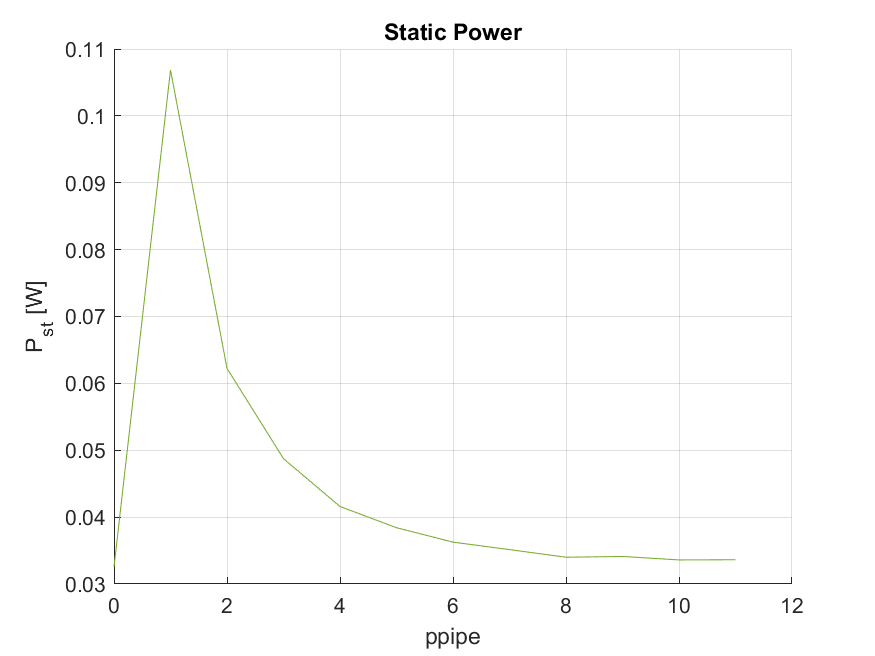
\includegraphics[width=9cm]{immagini/radix2ppipe2/p_static_pipe.png}
		\end{subfigure}
	}
{
		\begin{subfigure}{0.55\textwidth}
			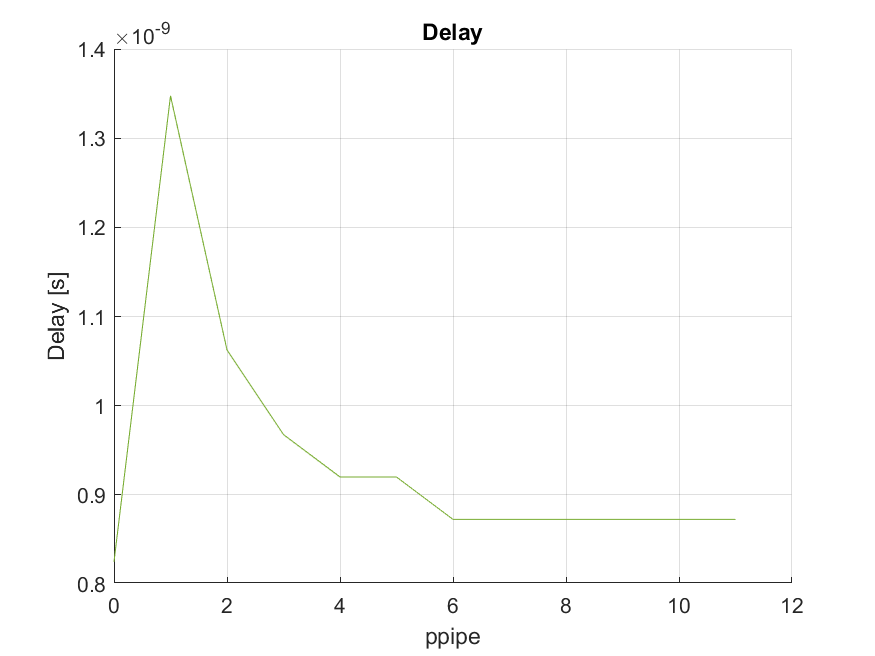
\includegraphics[width=9cm]{immagini/radix2ppipe2/delay_pipe.png}
		\end{subfigure}
		\begin{subfigure}{0.55\textwidth}
			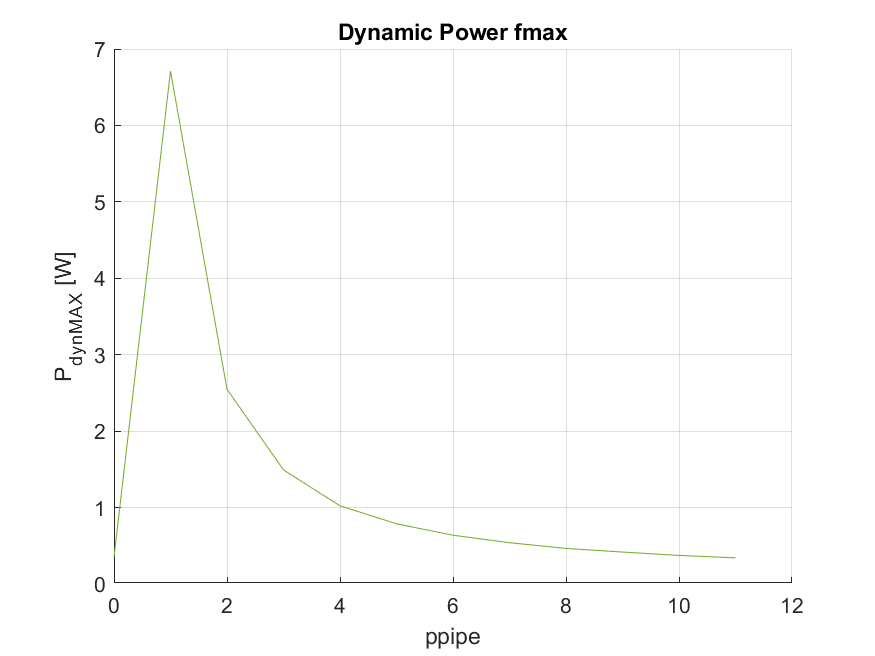
\includegraphics[width=9cm]{immagini/radix2ppipe2/p_dyn_fmax_pipe.png}
		\end{subfigure}
	}
	\caption{Comparisons}
	\label{fig:ppipe}
\end{figure}
Considering the delay, in particular it is possible to notice how the behaviour does not strictly follow the one of the other 3 plots presented. The trend in this case is linked to the number of operands which determine the number of the levels of the tree. In this case since for 128 operands the number of levels is 11, starting from ppipe=6 the trend is perfectly flat: only one pipe level is inserted for ppipe$>$6 therefore the total delay of the tree is the same. Something similar happens for ppipe=4 and ppipe=5 but 2 register levels are added in this case.
It is therefore possible to notice how the optimal pipe percentage to be inserted in the tree depends on the number of operands.

\subsubsection{Throughput} In Figure \ref{fmax} is reported the throughput taking into account different pipeline depths cases. 

The trend is similar to the previous cases: the fully pipelined case (ppipe=1) is characterized by the highest possible throughput since the critical path is the one of a single FA. This allows to have multiple elaborations in execution at the same time (at different stages of the pipelined structure). With an increasing number of pipeline stages, latency (in terms of clock cycles needed to complete an elaboration) increases as well. 

\begin{figure}[H]
	\centering
	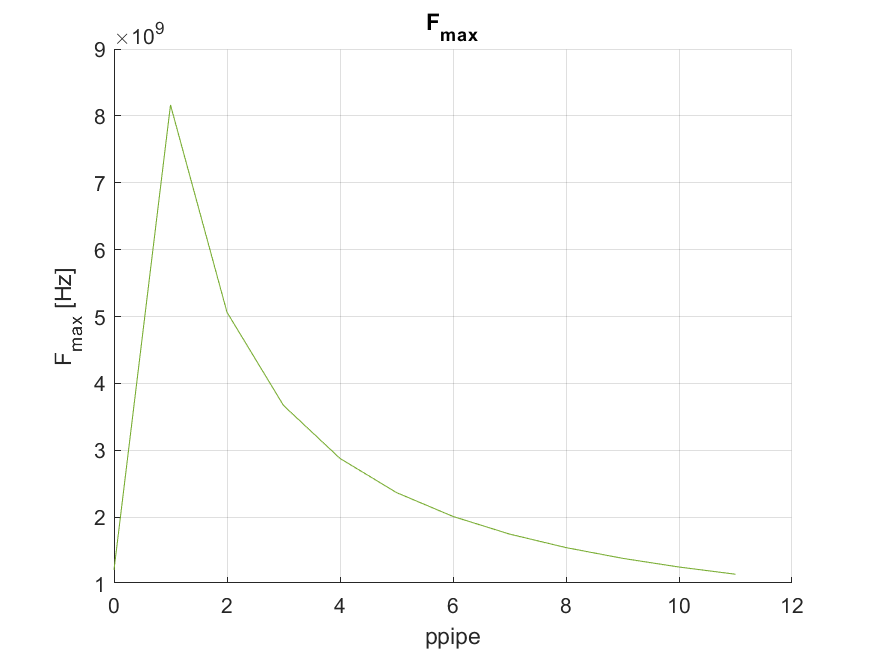
\includegraphics[width=10cm]{immagini/radix2ppipe2/fmax_pipe.png}
	\caption{Maximum throughput for different pipeline depths}
	\label{fmax}
\end{figure}
   
\subsection{VHDL}
The developed script also generates the VHDL description of the tree. The output design has been then verified through simulation. In Fig \ref{fig:schem} is shown the block diagram schematic for a simple tree with n=4, k=4 and ppipe=2.  

\begin{figure}[H]
	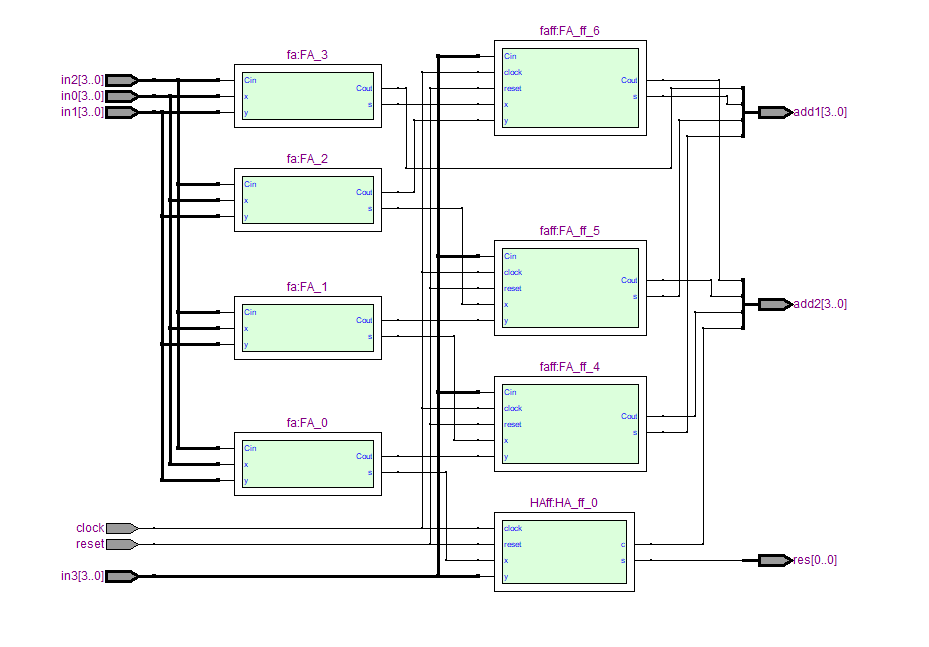
\includegraphics[trim={0 1.2cm 0 0},clip=true,scale=0.8]{./immagini/4x4.png}
	\caption{4x4 Wallace tree design (ppipe=2)}
	\label{fig:schem}
\end{figure}

The flip flop layer is placed after the second level of the tree, it has been included in the components $HA\_ff$ and $FA\_ff$.

\section{Conclusions}
It was developed a model of a Wallace tree with a percentage of pipelining which can be defined by the user. The present model also allows to not insert any pipeline stage. 
The main advantage of a pipelined implemantation lies in the fact that throughput increases while the time required to complete a single computation increases. 
Since flip flop insertion causes an increase of both area and power, it is therefore important to carefully choose how many pipeline stages should be inserted in the tree. 
The choice depends on the application, the optimal choice for the Wallace tree does not corresponds to a fully pipelined approach since it maximizes occupied area, consumptions and also latency.





